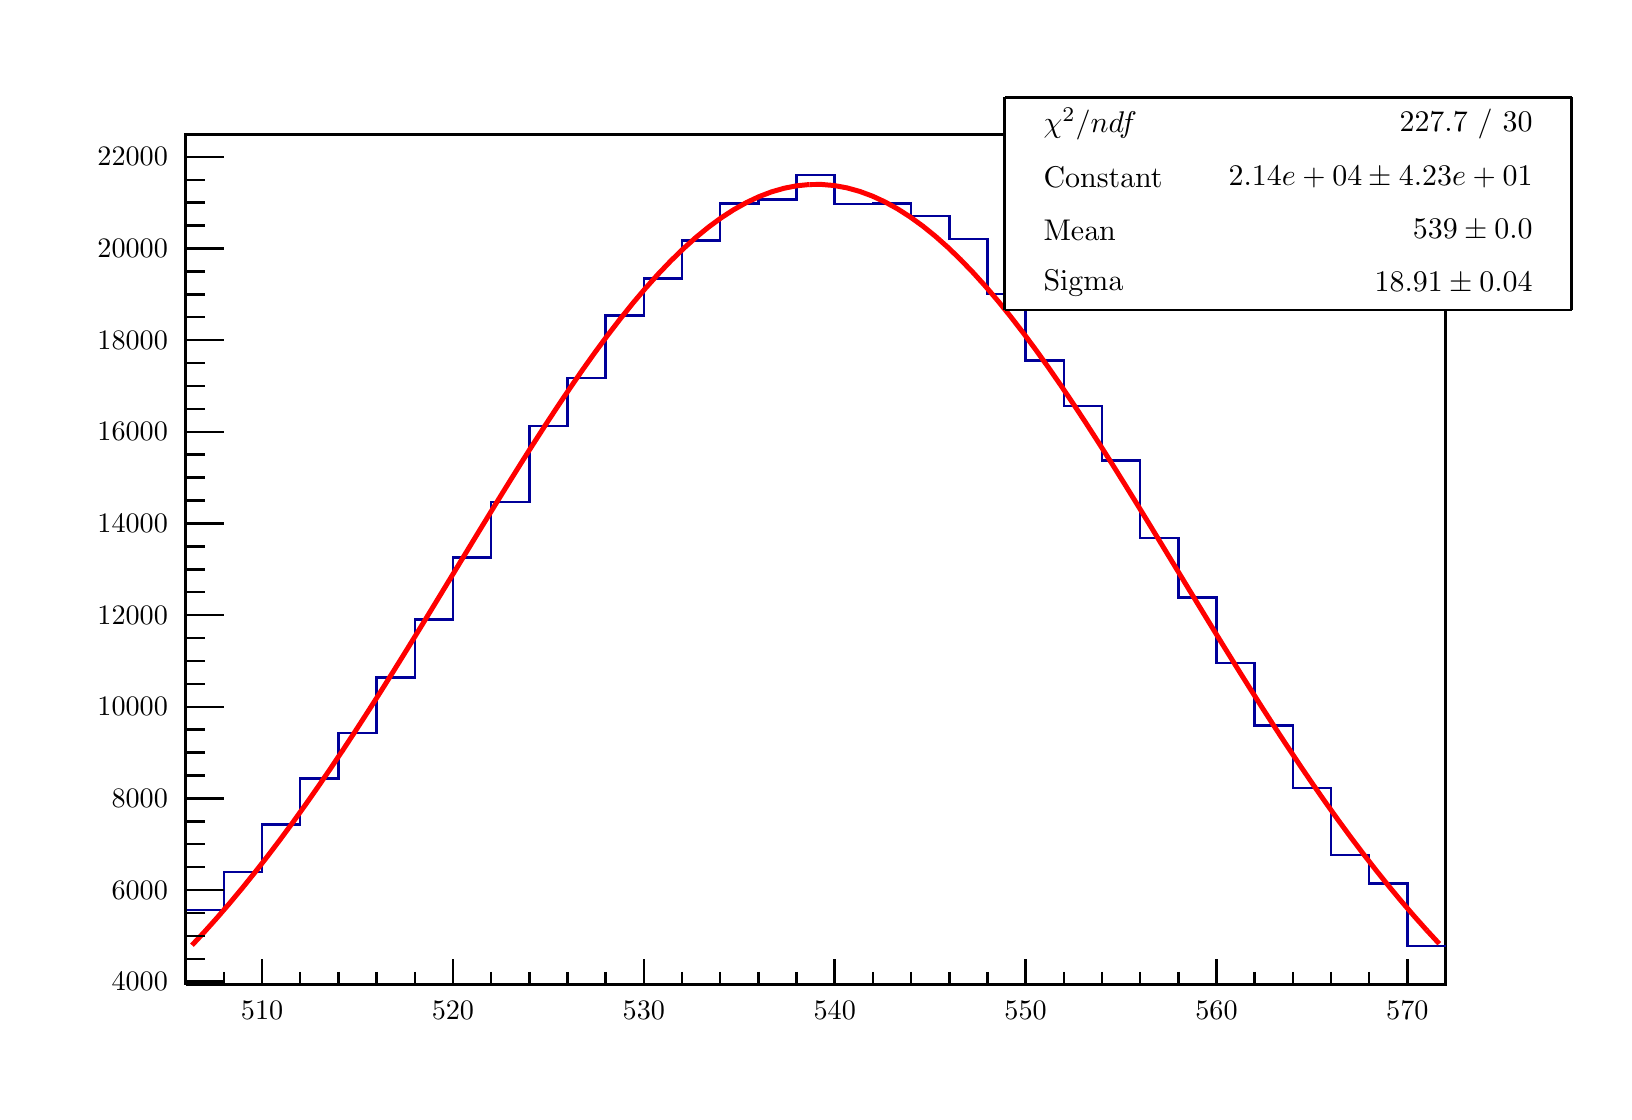
\begin{tikzpicture}
\pgfdeclareplotmark{cross} {
\pgfpathmoveto{\pgfpoint{-0.3\pgfplotmarksize}{\pgfplotmarksize}}
\pgfpathlineto{\pgfpoint{+0.3\pgfplotmarksize}{\pgfplotmarksize}}
\pgfpathlineto{\pgfpoint{+0.3\pgfplotmarksize}{0.3\pgfplotmarksize}}
\pgfpathlineto{\pgfpoint{+1\pgfplotmarksize}{0.3\pgfplotmarksize}}
\pgfpathlineto{\pgfpoint{+1\pgfplotmarksize}{-0.3\pgfplotmarksize}}
\pgfpathlineto{\pgfpoint{+0.3\pgfplotmarksize}{-0.3\pgfplotmarksize}}
\pgfpathlineto{\pgfpoint{+0.3\pgfplotmarksize}{-1.\pgfplotmarksize}}
\pgfpathlineto{\pgfpoint{-0.3\pgfplotmarksize}{-1.\pgfplotmarksize}}
\pgfpathlineto{\pgfpoint{-0.3\pgfplotmarksize}{-0.3\pgfplotmarksize}}
\pgfpathlineto{\pgfpoint{-1.\pgfplotmarksize}{-0.3\pgfplotmarksize}}
\pgfpathlineto{\pgfpoint{-1.\pgfplotmarksize}{0.3\pgfplotmarksize}}
\pgfpathlineto{\pgfpoint{-0.3\pgfplotmarksize}{0.3\pgfplotmarksize}}
\pgfpathclose
\pgfusepathqstroke
}
\pgfdeclareplotmark{cross*} {
\pgfpathmoveto{\pgfpoint{-0.3\pgfplotmarksize}{\pgfplotmarksize}}
\pgfpathlineto{\pgfpoint{+0.3\pgfplotmarksize}{\pgfplotmarksize}}
\pgfpathlineto{\pgfpoint{+0.3\pgfplotmarksize}{0.3\pgfplotmarksize}}
\pgfpathlineto{\pgfpoint{+1\pgfplotmarksize}{0.3\pgfplotmarksize}}
\pgfpathlineto{\pgfpoint{+1\pgfplotmarksize}{-0.3\pgfplotmarksize}}
\pgfpathlineto{\pgfpoint{+0.3\pgfplotmarksize}{-0.3\pgfplotmarksize}}
\pgfpathlineto{\pgfpoint{+0.3\pgfplotmarksize}{-1.\pgfplotmarksize}}
\pgfpathlineto{\pgfpoint{-0.3\pgfplotmarksize}{-1.\pgfplotmarksize}}
\pgfpathlineto{\pgfpoint{-0.3\pgfplotmarksize}{-0.3\pgfplotmarksize}}
\pgfpathlineto{\pgfpoint{-1.\pgfplotmarksize}{-0.3\pgfplotmarksize}}
\pgfpathlineto{\pgfpoint{-1.\pgfplotmarksize}{0.3\pgfplotmarksize}}
\pgfpathlineto{\pgfpoint{-0.3\pgfplotmarksize}{0.3\pgfplotmarksize}}
\pgfpathclose
\pgfusepathqfillstroke
}
\pgfdeclareplotmark{newstar} {
\pgfpathmoveto{\pgfqpoint{0pt}{\pgfplotmarksize}}
\pgfpathlineto{\pgfqpointpolar{44}{0.5\pgfplotmarksize}}
\pgfpathlineto{\pgfqpointpolar{18}{\pgfplotmarksize}}
\pgfpathlineto{\pgfqpointpolar{-20}{0.5\pgfplotmarksize}}
\pgfpathlineto{\pgfqpointpolar{-54}{\pgfplotmarksize}}
\pgfpathlineto{\pgfqpointpolar{-90}{0.5\pgfplotmarksize}}
\pgfpathlineto{\pgfqpointpolar{234}{\pgfplotmarksize}}
\pgfpathlineto{\pgfqpointpolar{198}{0.5\pgfplotmarksize}}
\pgfpathlineto{\pgfqpointpolar{162}{\pgfplotmarksize}}
\pgfpathlineto{\pgfqpointpolar{134}{0.5\pgfplotmarksize}}
\pgfpathclose
\pgfusepathqstroke
}
\pgfdeclareplotmark{newstar*} {
\pgfpathmoveto{\pgfqpoint{0pt}{\pgfplotmarksize}}
\pgfpathlineto{\pgfqpointpolar{44}{0.5\pgfplotmarksize}}
\pgfpathlineto{\pgfqpointpolar{18}{\pgfplotmarksize}}
\pgfpathlineto{\pgfqpointpolar{-20}{0.5\pgfplotmarksize}}
\pgfpathlineto{\pgfqpointpolar{-54}{\pgfplotmarksize}}
\pgfpathlineto{\pgfqpointpolar{-90}{0.5\pgfplotmarksize}}
\pgfpathlineto{\pgfqpointpolar{234}{\pgfplotmarksize}}
\pgfpathlineto{\pgfqpointpolar{198}{0.5\pgfplotmarksize}}
\pgfpathlineto{\pgfqpointpolar{162}{\pgfplotmarksize}}
\pgfpathlineto{\pgfqpointpolar{134}{0.5\pgfplotmarksize}}
\pgfpathclose
\pgfusepathqfillstroke
}
\definecolor{c}{rgb}{1,1,1};
\draw [color=c, fill=c] (0,0) rectangle (20,13.4957);
\draw [color=c, fill=c] (2,1.34957) rectangle (18,12.1461);
\definecolor{c}{rgb}{0,0,0};
\draw [c,line width=0.9] (2,1.34957) -- (2,12.1461) -- (18,12.1461) -- (18,1.34957) -- (2,1.34957);
\definecolor{c}{rgb}{1,1,1};
\draw [color=c, fill=c] (2,1.34957) rectangle (18,12.1461);
\definecolor{c}{rgb}{0,0,0};
\draw [c,line width=0.9] (2,1.34957) -- (2,12.1461) -- (18,12.1461) -- (18,1.34957) -- (2,1.34957);
\definecolor{c}{rgb}{0,0,0.6};
\draw [c,line width=0.9] (2,2.29722) -- (2.48485,2.29722) -- (2.48485,2.78025) -- (2.9697,2.78025) -- (2.9697,3.38609) -- (3.45455,3.38609) -- (3.45455,3.9698) -- (3.93939,3.9698) -- (3.93939,4.54537) -- (4.42424,4.54537) -- (4.42424,5.25071) --
 (4.90909,5.25071) -- (4.90909,5.98574) -- (5.39394,5.98574) -- (5.39394,6.77548) -- (5.87879,6.77548) -- (5.87879,7.48082) -- (6.36364,7.48082) -- (6.36364,8.44107) -- (6.84848,8.44107) -- (6.84848,9.05563) -- (7.33333,9.05563) -- (7.33333,9.84653)
 -- (7.81818,9.84653) -- (7.81818,10.3185) -- (8.30303,10.3185) -- (8.30303,10.7986) -- (8.78788,10.7986) -- (8.78788,11.27) -- (9.27273,11.27) -- (9.27273,11.323) -- (9.75758,11.323) -- (9.75758,11.632) -- (10.2424,11.632) -- (10.2424,11.2619) --
 (10.7273,11.2619) -- (10.7273,11.2671) -- (11.2121,11.2671) -- (11.2121,11.11) -- (11.697,11.11) -- (11.697,10.8196) -- (12.1818,10.8196) -- (12.1818,10.1171) -- (12.6667,10.1171) -- (12.6667,9.27503) -- (13.1515,9.27503) -- (13.1515,8.69947) --
 (13.6364,8.69947) -- (13.6364,8.00285) -- (14.1212,8.00285) -- (14.1212,7.02398) -- (14.6061,7.02398) -- (14.6061,6.26742) -- (15.0909,6.26742) -- (15.0909,5.43694) -- (15.5758,5.43694) -- (15.5758,4.6379) -- (16.0606,4.6379) -- (16.0606,3.84351) --
 (16.5455,3.84351) -- (16.5455,2.99442) -- (17.0303,2.99442) -- (17.0303,2.63302) -- (17.5152,2.63302) -- (17.5152,1.83921) -- (18,1.83921);
\definecolor{c}{rgb}{1,0,0};
\draw [c,line width=1.8] (2.08,1.84973) -- (2.24,2.02159) -- (2.4,2.2002) -- (2.56,2.38553) -- (2.72,2.5775) -- (2.88,2.77601) -- (3.04,2.98095) -- (3.2,3.19214) -- (3.36,3.4094) -- (3.52,3.63251) -- (3.68,3.8612) -- (3.84,4.09519) -- (4,4.33415) --
 (4.16,4.57773) -- (4.32,4.82551) -- (4.48,5.07709) -- (4.64,5.332) -- (4.8,5.58974) -- (4.96,5.84979) -- (5.12,6.11161) -- (5.28,6.3746) -- (5.44,6.63816) -- (5.6,6.90165) -- (5.76,7.16442) -- (5.92,7.4258) -- (6.08,7.6851) -- (6.24,7.9416) --
 (6.4,8.1946) -- (6.56,8.44336) -- (6.72,8.68716) -- (6.88,8.92527) -- (7.04,9.15696) -- (7.2,9.38151) -- (7.36,9.59821) -- (7.52,9.80635) -- (7.68,10.0053) -- (7.84,10.1943) -- (8,10.3728) -- (8.16,10.5402) -- (8.32,10.6958) -- (8.48,10.8392) --
 (8.64,10.9699) -- (8.8,11.0873) -- (8.96,11.1912) -- (9.12,11.281) -- (9.28,11.3565) -- (9.44,11.4174) -- (9.6,11.4635) -- (9.76,11.4946) -- (9.92,11.5106);
\draw [c,line width=1.8] (9.92,11.5106) -- (10.08,11.5114) -- (10.24,11.4971) -- (10.4,11.4677) -- (10.56,11.4232) -- (10.72,11.364) -- (10.88,11.2901) -- (11.04,11.2018) -- (11.2,11.0995) -- (11.36,10.9836) -- (11.52,10.8544) -- (11.68,10.7124) --
 (11.84,10.558) -- (12,10.3919) -- (12.16,10.2147) -- (12.32,10.0268) -- (12.48,9.82892) -- (12.64,9.62176) -- (12.8,9.40598) -- (12.96,9.18227) -- (13.12,8.95134) -- (13.28,8.71391) -- (13.44,8.4707) -- (13.6,8.22245) -- (13.76,7.96989) --
 (13.92,7.71374) -- (14.08,7.45472) -- (14.24,7.19354) -- (14.4,6.93089) -- (14.56,6.66744) -- (14.72,6.40386) -- (14.88,6.14077) -- (15.04,5.8788) -- (15.2,5.61852) -- (15.36,5.3605) -- (15.52,5.10525) -- (15.68,4.85328) -- (15.84,4.60505) --
 (16,4.36099) -- (16.16,4.1215) -- (16.32,3.88694) -- (16.48,3.65764) -- (16.64,3.4339) -- (16.8,3.21598) -- (16.96,3.0041) -- (17.12,2.79846) -- (17.28,2.59923) -- (17.44,2.40653) -- (17.6,2.22046) -- (17.76,2.0411);
\draw [c,line width=1.8] (17.76,2.0411) -- (17.92,1.86848);
\definecolor{c}{rgb}{1,1,1};
\draw [color=c, fill=c] (12.4,9.91934) rectangle (19.6,12.6185);
\definecolor{c}{rgb}{0,0,0};
\draw [c,line width=0.9] (12.4,9.91934) -- (19.6,9.91934);
\draw [c,line width=0.9] (19.6,9.91934) -- (19.6,12.6185);
\draw [c,line width=0.9] (19.6,12.6185) -- (12.4,12.6185);
\draw [c,line width=0.9] (12.4,12.6185) -- (12.4,9.91934);
\draw [anchor= west] (12.76,12.2811) node[scale=1.08185, color=c, rotate=0]{$\chi^{2} / ndf $};
\draw [anchor= east] (19.24,12.2811) node[scale=1.08185, color=c, rotate=0]{ 227.7 / 30};
\draw [anchor= west] (12.76,11.6063) node[scale=1.08185, color=c, rotate=0]{Constant };
\draw [anchor= east] (19.24,11.6063) node[scale=1.08185, color=c, rotate=0]{$ 2.14e+04 \pm 4.23e+01$};
\draw [anchor= west] (12.76,10.9315) node[scale=1.08185, color=c, rotate=0]{Mean     };
\draw [anchor= east] (19.24,10.9315) node[scale=1.08185, color=c, rotate=0]{$   539 \pm 0.0$};
\draw [anchor= west] (12.76,10.2567) node[scale=1.08185, color=c, rotate=0]{Sigma    };
\draw [anchor= east] (19.24,10.2567) node[scale=1.08185, color=c, rotate=0]{$ 18.91 \pm 0.04$};
\draw [c,line width=0.9] (2,1.34957) -- (18,1.34957);
\draw [c,line width=0.9] (2.9697,1.67347) -- (2.9697,1.34957);
\draw [c,line width=0.9] (3.45455,1.51152) -- (3.45455,1.34957);
\draw [c,line width=0.9] (3.93939,1.51152) -- (3.93939,1.34957);
\draw [c,line width=0.9] (4.42424,1.51152) -- (4.42424,1.34957);
\draw [c,line width=0.9] (4.90909,1.51152) -- (4.90909,1.34957);
\draw [c,line width=0.9] (5.39394,1.67347) -- (5.39394,1.34957);
\draw [c,line width=0.9] (5.87879,1.51152) -- (5.87879,1.34957);
\draw [c,line width=0.9] (6.36364,1.51152) -- (6.36364,1.34957);
\draw [c,line width=0.9] (6.84848,1.51152) -- (6.84848,1.34957);
\draw [c,line width=0.9] (7.33333,1.51152) -- (7.33333,1.34957);
\draw [c,line width=0.9] (7.81818,1.67347) -- (7.81818,1.34957);
\draw [c,line width=0.9] (8.30303,1.51152) -- (8.30303,1.34957);
\draw [c,line width=0.9] (8.78788,1.51152) -- (8.78788,1.34957);
\draw [c,line width=0.9] (9.27273,1.51152) -- (9.27273,1.34957);
\draw [c,line width=0.9] (9.75758,1.51152) -- (9.75758,1.34957);
\draw [c,line width=0.9] (10.2424,1.67347) -- (10.2424,1.34957);
\draw [c,line width=0.9] (10.7273,1.51152) -- (10.7273,1.34957);
\draw [c,line width=0.9] (11.2121,1.51152) -- (11.2121,1.34957);
\draw [c,line width=0.9] (11.697,1.51152) -- (11.697,1.34957);
\draw [c,line width=0.9] (12.1818,1.51152) -- (12.1818,1.34957);
\draw [c,line width=0.9] (12.6667,1.67347) -- (12.6667,1.34957);
\draw [c,line width=0.9] (13.1515,1.51152) -- (13.1515,1.34957);
\draw [c,line width=0.9] (13.6364,1.51152) -- (13.6364,1.34957);
\draw [c,line width=0.9] (14.1212,1.51152) -- (14.1212,1.34957);
\draw [c,line width=0.9] (14.6061,1.51152) -- (14.6061,1.34957);
\draw [c,line width=0.9] (15.0909,1.67347) -- (15.0909,1.34957);
\draw [c,line width=0.9] (15.5758,1.51152) -- (15.5758,1.34957);
\draw [c,line width=0.9] (16.0606,1.51152) -- (16.0606,1.34957);
\draw [c,line width=0.9] (16.5455,1.51152) -- (16.5455,1.34957);
\draw [c,line width=0.9] (17.0303,1.51152) -- (17.0303,1.34957);
\draw [c,line width=0.9] (17.5152,1.67347) -- (17.5152,1.34957);
\draw [c,line width=0.9] (2.9697,1.67347) -- (2.9697,1.34957);
\draw [c,line width=0.9] (2.48485,1.51152) -- (2.48485,1.34957);
\draw [c,line width=0.9] (2,1.51152) -- (2,1.34957);
\draw [c,line width=0.9] (17.5152,1.67347) -- (17.5152,1.34957);
\draw [c,line width=0.9] (18,1.51152) -- (18,1.34957);
\draw [anchor=base] (2.9697,0.904212) node[scale=1.01821, color=c, rotate=0]{510};
\draw [anchor=base] (5.39394,0.904212) node[scale=1.01821, color=c, rotate=0]{520};
\draw [anchor=base] (7.81818,0.904212) node[scale=1.01821, color=c, rotate=0]{530};
\draw [anchor=base] (10.2424,0.904212) node[scale=1.01821, color=c, rotate=0]{540};
\draw [anchor=base] (12.6667,0.904212) node[scale=1.01821, color=c, rotate=0]{550};
\draw [anchor=base] (15.0909,0.904212) node[scale=1.01821, color=c, rotate=0]{560};
\draw [anchor=base] (17.5152,0.904212) node[scale=1.01821, color=c, rotate=0]{570};
\draw [c,line width=0.9] (2,1.34957) -- (2,12.1461);
\draw [c,line width=0.9] (2.48,1.38644) -- (2,1.38644);
\draw [c,line width=0.9] (2.24,1.67742) -- (2,1.67742);
\draw [c,line width=0.9] (2.24,1.96841) -- (2,1.96841);
\draw [c,line width=0.9] (2.24,2.25939) -- (2,2.25939);
\draw [c,line width=0.9] (2.48,2.55038) -- (2,2.55038);
\draw [c,line width=0.9] (2.24,2.84136) -- (2,2.84136);
\draw [c,line width=0.9] (2.24,3.13235) -- (2,3.13235);
\draw [c,line width=0.9] (2.24,3.42333) -- (2,3.42333);
\draw [c,line width=0.9] (2.48,3.71432) -- (2,3.71432);
\draw [c,line width=0.9] (2.24,4.0053) -- (2,4.0053);
\draw [c,line width=0.9] (2.24,4.29629) -- (2,4.29629);
\draw [c,line width=0.9] (2.24,4.58727) -- (2,4.58727);
\draw [c,line width=0.9] (2.48,4.87825) -- (2,4.87825);
\draw [c,line width=0.9] (2.24,5.16924) -- (2,5.16924);
\draw [c,line width=0.9] (2.24,5.46022) -- (2,5.46022);
\draw [c,line width=0.9] (2.24,5.75121) -- (2,5.75121);
\draw [c,line width=0.9] (2.48,6.04219) -- (2,6.04219);
\draw [c,line width=0.9] (2.24,6.33318) -- (2,6.33318);
\draw [c,line width=0.9] (2.24,6.62416) -- (2,6.62416);
\draw [c,line width=0.9] (2.24,6.91515) -- (2,6.91515);
\draw [c,line width=0.9] (2.48,7.20613) -- (2,7.20613);
\draw [c,line width=0.9] (2.24,7.49712) -- (2,7.49712);
\draw [c,line width=0.9] (2.24,7.7881) -- (2,7.7881);
\draw [c,line width=0.9] (2.24,8.07909) -- (2,8.07909);
\draw [c,line width=0.9] (2.48,8.37007) -- (2,8.37007);
\draw [c,line width=0.9] (2.24,8.66106) -- (2,8.66106);
\draw [c,line width=0.9] (2.24,8.95204) -- (2,8.95204);
\draw [c,line width=0.9] (2.24,9.24302) -- (2,9.24302);
\draw [c,line width=0.9] (2.48,9.53401) -- (2,9.53401);
\draw [c,line width=0.9] (2.24,9.82499) -- (2,9.82499);
\draw [c,line width=0.9] (2.24,10.116) -- (2,10.116);
\draw [c,line width=0.9] (2.24,10.407) -- (2,10.407);
\draw [c,line width=0.9] (2.48,10.6979) -- (2,10.6979);
\draw [c,line width=0.9] (2.24,10.9889) -- (2,10.9889);
\draw [c,line width=0.9] (2.24,11.2799) -- (2,11.2799);
\draw [c,line width=0.9] (2.24,11.5709) -- (2,11.5709);
\draw [c,line width=0.9] (2.48,11.8619) -- (2,11.8619);
\draw [c,line width=0.9] (2.48,1.38644) -- (2,1.38644);
\draw [c,line width=0.9] (2.48,11.8619) -- (2,11.8619);
\draw [anchor= east] (1.9,1.38644) node[scale=1.01821, color=c, rotate=0]{4000};
\draw [anchor= east] (1.9,2.55038) node[scale=1.01821, color=c, rotate=0]{6000};
\draw [anchor= east] (1.9,3.71432) node[scale=1.01821, color=c, rotate=0]{8000};
\draw [anchor= east] (1.9,4.87825) node[scale=1.01821, color=c, rotate=0]{10000};
\draw [anchor= east] (1.9,6.04219) node[scale=1.01821, color=c, rotate=0]{12000};
\draw [anchor= east] (1.9,7.20613) node[scale=1.01821, color=c, rotate=0]{14000};
\draw [anchor= east] (1.9,8.37007) node[scale=1.01821, color=c, rotate=0]{16000};
\draw [anchor= east] (1.9,9.53401) node[scale=1.01821, color=c, rotate=0]{18000};
\draw [anchor= east] (1.9,10.6979) node[scale=1.01821, color=c, rotate=0]{20000};
\draw [anchor= east] (1.9,11.8619) node[scale=1.01821, color=c, rotate=0]{22000};
\definecolor{c}{rgb}{1,1,1};
\draw [color=c, fill=c] (12.4,9.91934) rectangle (19.6,12.6185);
\definecolor{c}{rgb}{0,0,0};
\draw [c,line width=0.9] (12.4,9.91934) -- (19.6,9.91934);
\draw [c,line width=0.9] (19.6,9.91934) -- (19.6,12.6185);
\draw [c,line width=0.9] (19.6,12.6185) -- (12.4,12.6185);
\draw [c,line width=0.9] (12.4,12.6185) -- (12.4,9.91934);
\draw [anchor= west] (12.76,12.2811) node[scale=1.08185, color=c, rotate=0]{$\chi^{2} / ndf $};
\draw [anchor= east] (19.24,12.2811) node[scale=1.08185, color=c, rotate=0]{ 227.7 / 30};
\draw [anchor= west] (12.76,11.6063) node[scale=1.08185, color=c, rotate=0]{Constant };
\draw [anchor= east] (19.24,11.6063) node[scale=1.08185, color=c, rotate=0]{$ 2.14e+04 \pm 4.23e+01$};
\draw [anchor= west] (12.76,10.9315) node[scale=1.08185, color=c, rotate=0]{Mean     };
\draw [anchor= east] (19.24,10.9315) node[scale=1.08185, color=c, rotate=0]{$   539 \pm 0.0$};
\draw [anchor= west] (12.76,10.2567) node[scale=1.08185, color=c, rotate=0]{Sigma    };
\draw [anchor= east] (19.24,10.2567) node[scale=1.08185, color=c, rotate=0]{$ 18.91 \pm 0.04$};
\end{tikzpicture}
